\documentclass[tikz,border=10pt]{standalone}
\usepackage[scaled]{helvet} % Load Helvetica font
\renewcommand*\familydefault{\sfdefault} % Set the default font to the sans serif family

\begin{document}


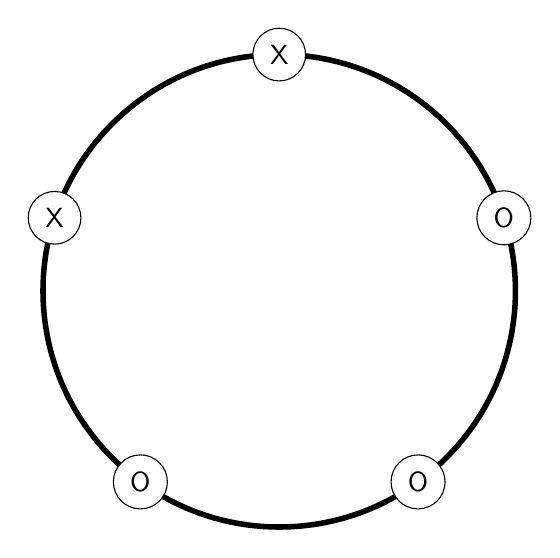
\begin{tikzpicture}
  % Define radius
  \def \radius {3cm}
  
  % Draw the main circle
  \draw[line width=2] (0,0) circle (\radius);
  
  % Draw the points on the circle and label them
  \node[draw, circle, fill=white] at ({ pi/2 * 180/pi }:\radius) {X};
  \node[draw, circle, fill=white] at ({ (1*(2*pi/5) + pi/2 )* 180/pi }:\radius) {X};
  \node[draw, circle, fill=white] at ({ (2*(2*pi/5) + pi/2 )* 180/pi }:\radius) {O};
  \node[draw, circle, fill=white] at ({ (3*(2*pi/5) + pi/2 )* 180/pi }:\radius) {O};
  \node[draw, circle, fill=white] at ({ (4*(2*pi/5) + pi/2 )* 180/pi }:\radius) {O};

\end{tikzpicture}



\end{document}

